% MindBox Companion — System Architecture (Student Guide)
% Compile with: pdflatex MindBox-System-Architecture.tex (run twice for TOC)
% Optional: install a LaTeX distribution (TeX Live, MiKTeX, or Overleaf)

\documentclass[11pt,a4paper]{article}

\usepackage[utf8]{inputenc}
\usepackage[T1]{fontenc}
\usepackage{lmodern}
\usepackage[margin=2.5cm]{geometry}
\usepackage{graphicx}
\usepackage{hyperref}
\usepackage{xcolor}
\usepackage{booktabs}
\usepackage{longtable}
\usepackage{enumitem}
\usepackage{listings}
\usepackage{tikz}
\usetikzlibrary{arrows.meta, positioning, shapes.geometric, fit, backgrounds}

\hypersetup{
  colorlinks=true,
  linkcolor=blue!70!black,
  urlcolor=blue!70!black,
  citecolor=blue!70!black
}

\definecolor{codebg}{RGB}{245,245,245}
\definecolor{keyword}{RGB}{0,80,160}

\lstset{
  basicstyle=\ttfamily\small,
  backgroundcolor=\color{codebg},
  frame=single,
  rulecolor=\color{gray!40},
  breaklines=true,
  columns=fullflexible,
  showstringspaces=false
}

\newcommand{\keyword}[1]{\textbf{\textcolor{keyword}{#1}}}
\newcommand{\filepath}[1]{\texttt{#1}}
\newcommand{\concept}[2]{\textbf{#1} --- #2}

\title{\textbf{MindBox Companion}\\[0.4em]
\large A Student-Friendly Guide to the System Architecture}
\author{Study Assistor Project (IoT Focus Device + Web App)}
\date{\today}

\begin{document}
\maketitle

\begin{abstract}
This document explains how the \textbf{MindBox Companion} web application is built and how it connects to the physical MindBox device and cloud database. It is written for computer science students: technical terms are defined when they first appear, and the focus is on \emph{how data moves} and \emph{why the code is organized} the way it is. No prior experience with our exact tools is required.
\end{abstract}

\tableofcontents
\newpage

%==============================================================================
\section{What Is This Project?}
%==============================================================================

The MindBox project has \textbf{two main parts}:

\begin{enumerate}[leftmargin=*]
  \item \textbf{The physical device (ESP32 microcontroller)} --- a small computer on a desk that runs a timer, reads sensors (noise, light, temperature, presence), shows status on LEDs, and sends session data over Wi-Fi.
  \item \textbf{The companion web app (this repository)} --- a website you open in a browser to sign in, see your focus history, charts, friends, reviewers, exports, and device status.
\end{enumerate}

Think of it like a fitness tracker: the \emph{device} collects data; the \emph{app} helps you understand and share that data. The app does \textbf{not} start or stop focus sessions for you --- that happens on the box (by design).

The web app lives in the folder \filepath{mindbox-companion-forge-main}. The firmware lives elsewhere in the parent project (\filepath{ESP32/}).

%==============================================================================
\section{Glossary: Keywords Explained Simply}
%==============================================================================

Before diving in, here is a mini-dictionary. Refer back to this section whenever a word feels unfamiliar.

\begin{longtable}{@{}p{3.2cm}p{10.5cm}@{}}
\toprule
\textbf{Term} & \textbf{Plain meaning} \\
\midrule
\endhead

Frontend &
The part that runs in the \textbf{browser}: buttons, pages, charts. Written in React (JavaScript/TypeScript UI library). \\

Backend &
The part that runs on a \textbf{server}: secure operations, talking to email services, accepting data from the device. In this project, much of the ``backend'' is actually \textbf{Supabase} (see below), not custom code we wrote from scratch. \\

Full-stack &
A project that includes \textbf{both} frontend and backend in one codebase. You work on UI and server logic in the same repository. \\

Monolith &
One application deployed as a \textbf{single unit} (one build, one server process), as opposed to many small microservices. Simpler for a student team. \\

SSR (Server-Side Rendering) &
The server can send \textbf{HTML already filled in} to the browser, not just an empty page that loads data later. Helps first load and SEO. \\

SPA (Single Page Application) &
After the first load, navigating between pages feels instant because JavaScript swaps content without full page reloads. TanStack Router gives us file-based pages with SPA behavior. \\

API &
Application Programming Interface: a defined way for programs to talk to each other (e.g.\ ``send JSON here, get JSON back''). \\

REST / HTTP routes &
URLs like \filepath{/ingest/sessions} that accept \keyword{POST} requests with JSON bodies. Our device uses two such routes. \\

Supabase &
A cloud service that gives us: (1) a \textbf{PostgreSQL database}, (2) \textbf{user login} (email + Google), (3) \textbf{security rules} (RLS). We do not run our own database server. \\

PostgreSQL &
A relational database (tables with rows and columns), like you may have seen in a databases course. \\

RLS (Row-Level Security) &
Database rules of the form: ``User Alice can only \textbf{read rows where user\_id = Alice's id}.'' Enforced \textbf{inside the database}, not only in our app code. \\

Auth / JWT / Session &
When you log in, Supabase gives the browser a \textbf{session} (stored in cookies). Every request proves ``I am this user.'' \\

OAuth / Google sign-in &
Instead of typing a password, you click ``Continue with Google''; Google confirms your identity; Supabase creates or finds your account. \\

Anon key &
A \textbf{public} API key safe to put in browser code because RLS limits what it can do. \\

Service-role key &
A \textbf{secret} key that bypasses RLS. Used only on the server for device ingest and admin tasks. \textbf{Never} expose it to the browser. \\

React &
A JavaScript library for building UIs from reusable \textbf{components} (functions that return HTML-like JSX). \\

TypeScript &
JavaScript with \textbf{types} (e.g.\ ``this variable is a string''). Catches many bugs before runtime. \\

Component &
A reusable piece of UI, e.g.\ a button, a chart, or the sidebar navigation. \\

Hook &
A React function starting with \texttt{use...} that lets components share logic (e.g.\ \texttt{useAuth}, \texttt{useSessions}). \\

Context &
A way to pass data (like ``current user'') through the component tree without prop-drilling every level. \\

TanStack Router &
Library that maps \textbf{URLs to page files}. File \filepath{routes/history.tsx} becomes URL \filepath{/history}. \\

TanStack Query &
Library that \textbf{caches} data fetched from the server (sessions, settings) and refetches when needed. Avoids redundant network calls. \\

TanStack Start &
Framework that combines React, routing, SSR, and \textbf{server functions} in one project. \\

Server function &
A TypeScript function marked with \texttt{createServerFn} that runs \textbf{only on the server} but can be called from the browser like a remote procedure call (RPC). \\

Vite &
Build tool: bundles TypeScript/React for production and provides a fast dev server during development. \\

Nitro &
Production server adapter (can deploy to cloud platforms). Wraps our app for hosting. \\

Zod &
Library to \textbf{validate} input shapes (e.g.\ ``email must look like an email''). Used on forms and server functions. \\

Migration &
A SQL script that changes the database schema (creates tables, policies). We run these manually in Supabase's SQL Editor. \\

RPC (in Supabase) &
A \textbf{stored procedure} in SQL, e.g.\ \texttt{get\_leaderboard()}, callable from the app like a function. \\

Idempotent &
Doing the same operation twice has the same effect as once. Device re-sending the same session does not create duplicates. \\

Ingest &
The process of the \textbf{device uploading} session and telemetry data to our server. \\

Telemetry &
Live device status: battery \%, Wi-Fi signal, sensor health, state (working / idle / warning). \\

Focus Load Estimate (FLE) &
A \textbf{heuristic score} 0--100 combining session progress, noise, light stability, and presence interruptions. \textbf{Not} a medical measurement --- always labeled as an estimate in the UI. \\

\bottomrule
\end{longtable}

%==============================================================================
\section{High-Level Architecture}
%==============================================================================

\subsection{The pattern we use}

Our project is best described as:

\begin{quote}
\textbf{A full-stack monolith with a Backend-as-a-Service (BaaS).}
\end{quote}

\begin{itemize}[leftmargin=*]
  \item \textbf{Monolith} = one codebase, one deployment.
  \item \textbf{BaaS} = Supabase handles most backend concerns (database + auth + security).
  \item \textbf{Thin custom server} = we add device ingest routes, email PDFs, and pairing logic on top.
\end{itemize}

This is \textbf{not} classic MVC (Model-View-Controller) in the textbook sense, and \textbf{not} microservices. It is closer to a modern ``React app + Supabase + a few server endpoints.''

\subsection{Architecture diagram}

\begin{center}
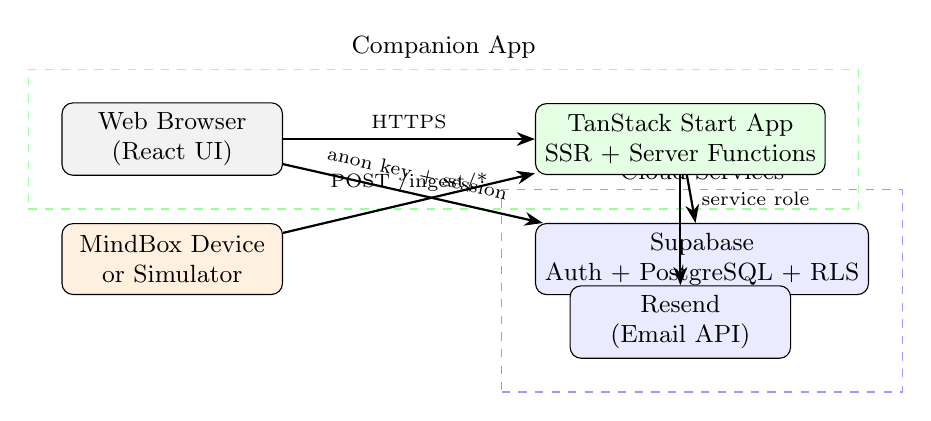
\begin{tikzpicture}[
  node distance=0.6cm and 1.2cm,
  box/.style={draw, rounded corners, minimum width=2.8cm, minimum height=0.9cm, align=center, font=\small},
  cloud/.style={box, fill=blue!8},
  app/.style={box, fill=green!10},
  device/.style={box, fill=orange!12},
  user/.style={box, fill=gray!10}
]
  \node[user] (browser) {Web Browser\\(React UI)};
  \node[device, below=of browser] (esp) {MindBox Device\\or Simulator};
  \node[app, right=3.2cm of browser] (tanstack) {TanStack Start App\\SSR + Server Functions};
  \node[cloud, right=3.2cm of esp] (supa) {Supabase\\Auth + PostgreSQL + RLS};
  \node[cloud, below=1.4cm of tanstack] (resend) {Resend\\(Email API)};

  \draw[-{Stealth}, thick] (browser) -- node[above, font=\scriptsize]{HTTPS} (tanstack);
  \draw[-{Stealth}, thick] (browser) -- node[above, font=\scriptsize, sloped]{anon key + session} (supa);
  \draw[-{Stealth}, thick] (esp) -- node[above, font=\scriptsize]{POST /ingest/*} (tanstack);
  \draw[-{Stealth}, thick] (tanstack) -- node[right, font=\scriptsize]{service role} (supa);
  \draw[-{Stealth}, thick] (tanstack) -- (resend);

  \begin{scope}[on background layer]
    \node[fit=(browser)(tanstack), draw=green!40, dashed, inner sep=12pt, label={[font=\small]above:Companion App}] {};
    \node[fit=(supa)(resend), draw=blue!40, dashed, inner sep=12pt, label={[font=\small]above:Cloud Services}] {};
  \end{scope}
\end{tikzpicture}
\end{center}

\subsection{Who talks to whom?}

\begin{enumerate}[leftmargin=*]
  \item \textbf{Browser $\rightarrow$ Supabase directly} for most reads/writes (sessions list, settings). The anon key is public; \keyword{RLS} ensures users only see allowed rows.
  \item \textbf{Browser $\rightarrow$ Server functions} for privileged actions (email PDF, claim device code, reviewer invites). Server checks auth and may use the secret service-role key.
  \item \textbf{Device $\rightarrow$ /ingest/* routes} with a shared secret header. No user login on the device --- trust is ``whoever knows the secret and device id.''
  \item \textbf{Server $\rightarrow$ Resend} to send emails (reports, reviewer invites).
  \item \textbf{Browser $\rightarrow$ Google (via Supabase)} for OAuth login.
\end{enumerate}

%==============================================================================
\section{Project Folder Structure}
%==============================================================================

Understanding \emph{where} code lives helps you find things quickly.

\subsection{Top level}

\begin{lstlisting}
mindbox-companion-forge-main/
  src/                 <- All application source code
  supabase/migrations/ <- SQL to create tables and security rules
  scripts/             <- CLI tools (fake device for testing)
  docs/                <- Documentation (including this file)
  .env.example         <- Template for secrets (copy to .env)
  package.json         <- Dependencies and npm scripts
\end{lstlisting}

\subsection{Inside \filepath{src/}}

\begin{table}[h]
\centering
\small
\begin{tabular}{@{}ll@{}}
\toprule
Folder / file & Purpose \\
\midrule
\filepath{server.ts} & First code that runs on the server for each HTTP request \\
\filepath{start.ts} & Security middleware (CSRF, error handling) \\
\filepath{router.tsx} & Creates the router and React Query client \\
\filepath{routes/} & One file per page (Dashboard, History, Login, \ldots) \\
\filepath{components/} & Reusable UI (sidebar, charts, banners) \\
\filepath{components/ui/} & Low-level widgets (Button, Card, Input) \\
\filepath{hooks/} & Shared React logic (\texttt{useSessionScope}, nudges) \\
\filepath{lib/} & Business logic, database clients, server-only code \\
\filepath{routeTree.gen.ts} & Auto-generated --- do not edit manually \\
\bottomrule
\end{tabular}
\caption{Core \filepath{src/} layout}
\end{table}

\subsection{Inside \filepath{src/lib/} (the ``brain'')}

\begin{itemize}[leftmargin=*]
  \item \filepath{auth/} --- Login state, Google OAuth helpers.
  \item \filepath{supabase/} --- \texttt{client.ts} (browser), \texttt{server.ts} (server + admin).
  \item \filepath{queries/} --- Functions that fetch data + React Query hooks.
  \item \filepath{api/} --- Server functions (\texttt{*.functions.ts}).
  \item \filepath{ingest/} --- Device upload handler.
  \item \filepath{email/} --- PDF generation and Resend email sending.
  \item \filepath{focus-load.ts}, \filepath{insights.ts}, \filepath{export.ts} --- Pure logic (easy to unit test).
\end{itemize}

\textbf{Rule of thumb:} Pages in \filepath{routes/} should stay thin; put reusable logic in \filepath{lib/}.

\subsection{Database migrations}

Files \filepath{0001\_init.sql} through \filepath{0005\_google\_oauth\_profile.sql} define:

\begin{itemize}[leftmargin=*]
  \item Tables (\texttt{profiles}, \texttt{sessions}, \texttt{devices}, \ldots)
  \item RLS policies (who can SELECT/INSERT/UPDATE/DELETE)
  \item Triggers (auto-create profile when user signs up)
  \item RPC functions (\texttt{get\_leaderboard}, \texttt{get\_focus\_streak}, \ldots)
\end{itemize}

You apply them in the Supabase Dashboard SQL Editor, in order.

%==============================================================================
\section{Technology Stack (What We Use and Why)}
%==============================================================================

\begin{table}[h]
\centering
\small
\begin{tabular}{@{}lll@{}}
\toprule
Layer & Technology & Why \\
\midrule
Language & TypeScript & Types + same language front and back \\
UI & React 19 & Component-based interfaces \\
Routing & TanStack Router & URL $\leftrightarrow$ files, type-safe links \\
Data fetching & TanStack Query & Cache, loading states, refetch \\
Styling & Tailwind CSS & Utility classes, fast layout \\
Components & Radix + shadcn/ui & Accessible buttons, dialogs, etc. \\
Charts & Recharts & History and insights graphs \\
Validation & Zod & Safe input on client and server \\
Framework & TanStack Start & SSR + server functions \\
Build & Vite & Dev server and production bundle \\
Database & Supabase (PostgreSQL) & Managed DB + auth + RLS \\
Email & Resend & Transactional email with attachments \\
PDF & Puppeteer + pdfkit & Turn HTML reports into PDF files \\
Tests & Vitest & Unit tests for pure logic \\
\bottomrule
\end{tabular}
\end{table}

%==============================================================================
\section{The Database (Conceptual Model)}
%==============================================================================

You do not need to memorize every column. Understand the \textbf{relationships}:

\begin{center}
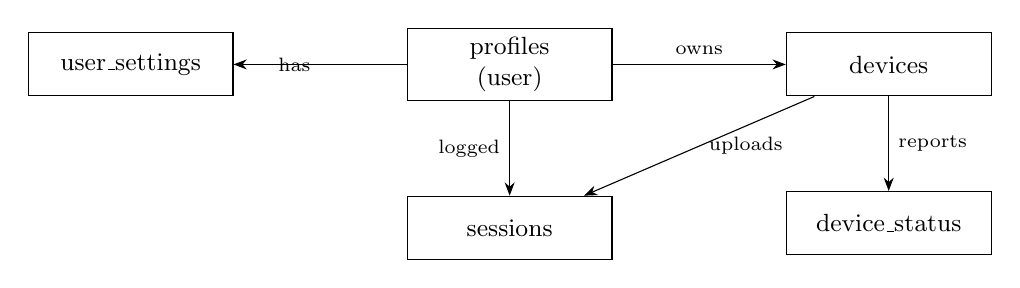
\begin{tikzpicture}[
  entity/.style={draw, rectangle, minimum width=2.6cm, minimum height=0.8cm, align=center, font=\small},
  rel/.style={-{Stealth}, font=\scriptsize}
]
  \node[entity] (user) {profiles\\(user)};
  \node[entity, right=2.2cm of user] (device) {devices};
  \node[entity, below=1.2cm of user] (session) {sessions};
  \node[entity, below=1.2cm of device] (status) {device\_status};
  \node[entity, left=2.2cm of user] (settings) {user\_settings};

  \draw[rel] (user) -- node[above]{owns} (device);
  \draw[rel] (user) -- node[left]{has} (settings);
  \draw[rel] (user) -- node[left]{logged} (session);
  \draw[rel] (device) -- node[right]{uploads} (session);
  \draw[rel] (device) -- node[right]{reports} (status);
\end{tikzpicture}
\end{center}

\textbf{Important tables:}

\begin{itemize}[leftmargin=*]
  \item \texttt{profiles} --- One row per signed-up user (name, email, daily goal).
  \item \texttt{sessions} --- Each focus block (start time, duration, mode, focus score, env averages).
  \item \texttt{focus\_load\_samples} / \texttt{env\_samples} --- Time-series points inside a session (for charts).
  \item \texttt{devices} + \texttt{device\_status} --- Which box belongs to whom; latest battery/Wi-Fi/state.
  \item \texttt{friendships} --- Social graph for leaderboard.
  \item \texttt{reviewer\_grants} --- Read-only access for teachers/parents.
  \item \texttt{user\_settings} --- Toggles (notifications, quiet hours, weekly email share).
\end{itemize}

%==============================================================================
\section{Data Flow: Step-by-Step Examples}
%==============================================================================

These walkthroughs answer: ``I clicked something --- what happens under the hood?''

%------------------------------------------------------------------------------
\subsection{Example A: Sign in with Google}
%------------------------------------------------------------------------------

\begin{enumerate}[leftmargin=*]
  \item User opens \filepath{/login} and clicks \textbf{Continue with Google}.
  \item Browser calls \texttt{signInWithGoogle()} in \filepath{lib/auth/google-oauth.ts}.
  \item Supabase redirects to Google; user picks an account.
  \item Google redirects back to Supabase, then to our app at \filepath{/auth/callback?code=...}.
  \item Page \filepath{auth/callback.tsx} exchanges the code for a \textbf{session} (cookies set).
  \item Database trigger \texttt{handle\_new\_user} creates \texttt{profiles} + \texttt{user\_settings} if new user.
  \item \filepath{AuthProvider} detects session; \filepath{AuthGate} in \filepath{\_\_root.tsx} allows access to the app shell.
  \item User lands on Dashboard; pages fetch data with their user id enforced by RLS.
\end{enumerate}

%------------------------------------------------------------------------------
\subsection{Example B: View session history}
%------------------------------------------------------------------------------

\begin{enumerate}[leftmargin=*]
  \item User navigates to \filepath{/history}.
  \item Component calls hook \texttt{useDailyAggregates(from, to)} from \filepath{queries/sessions.ts}.
  \item TanStack Query checks cache; if stale, runs \texttt{fetchSessions()}.
  \item \texttt{fetchSessions} uses \texttt{getSupabaseBrowserClient()} $\rightarrow$ SQL \texttt{SELECT * FROM sessions ORDER BY started\_at}.
  \item PostgreSQL applies \textbf{RLS}: only rows for this user (or reviewer-granted students) return.
  \item React renders bar/line charts (Recharts) and a session list.
  \item Date filters live in React state \textbf{and} URL search params for shareable links.
\end{enumerate}

%------------------------------------------------------------------------------
\subsection{Example C: Device uploads a session (real IoT path)}
%------------------------------------------------------------------------------

\begin{enumerate}[leftmargin=*]
  \item MindBox finishes a focus session; firmware builds JSON matching \filepath{focus-load.ts} types.
  \item Device POSTs to \filepath{https://your-app/ingest/sessions} with header \texttt{x-device-secret}.
  \item \filepath{server.ts} sees path \filepath{/ingest/sessions} and calls \filepath{ingest.server.ts} (skips normal page routing).
  \item Server validates secret, parses JSON with Zod, resolves \texttt{user\_id} from device ownership.
  \item Admin Supabase client \textbf{upserts} session row + sample rows (idempotent on device id + session id).
  \item User opens app; \texttt{useSessions} refetches; new session appears on Dashboard and History.
\end{enumerate}

%------------------------------------------------------------------------------
\subsection{Example D: Email a PDF report}
%------------------------------------------------------------------------------

\begin{enumerate}[leftmargin=*]
  \item User sets date range on \filepath{/exports}, clicks \textbf{Email PDF}.
  \item Browser calls server function \texttt{emailReport(\{ from, to \})}.
  \item Server verifies logged-in user via cookie session.
  \item \filepath{deliver-report.server.ts} loads sessions (admin client), builds HTML report, converts to PDF (Puppeteer).
  \item Finds recipient emails (user + active reviewers).
  \item Sends email via Resend API with PDF attached.
  \item UI shows success message with recipient list.
\end{enumerate}

%==============================================================================
\section{Application Entry Points}
%==============================================================================

``Where does execution start?'' depends on \textbf{dev vs production} and \textbf{browser vs server}.

\subsection{When you run \texttt{npm run dev}}

Vite starts a development server (usually \filepath{http://localhost:8080}). Each page load goes through TanStack Start's SSR pipeline.

\subsection{Production HTTP entry: \filepath{src/server.ts}}

Every incoming request hits \filepath{server.ts} first:

\begin{lstlisting}
if path is /ingest/sessions or /ingest/telemetry
  -> handle device upload (ingest.server.ts)
else
  -> TanStack SSR + React router (normal pages)
\end{lstlisting}

\subsection{React app entry: \filepath{src/routes/\_\_root.tsx}}

This file wraps the entire UI:

\begin{itemize}[leftmargin=*]
  \item Provides \texttt{QueryClientProvider} (TanStack Query).
  \item Provides \texttt{AuthProvider} (current user).
  \item \texttt{AuthGate} redirects guests to \filepath{/login} unless on a public page.
  \item Signed-in users see \texttt{AppShell} (sidebar + content).
\end{itemize}

\subsection{Files to read first (learning path)}

\begin{enumerate}[leftmargin=*]
  \item \filepath{routes/\_\_root.tsx} --- Auth and layout.
  \item \filepath{lib/auth/auth-context.tsx} --- Session lifecycle.
  \item \filepath{lib/supabase/client.ts} --- How the browser talks to the database.
  \item \filepath{lib/queries/sessions.ts} --- Main data loading.
  \item \filepath{routes/index.tsx} --- Dashboard.
  \item \filepath{lib/ingest/ingest.server.ts} --- Device integration.
  \item \filepath{supabase/migrations/0001\_init.sql} --- Schema and RLS.
\end{enumerate}

%==============================================================================
\section{State Management and Design Patterns}
%==============================================================================

\subsection{Where is ``state'' stored?}

\begin{table}[h]
\centering
\small
\begin{tabular}{@{}ll@{}}
\toprule
Kind of state & Mechanism \\
\midrule
Logged-in user & React Context (\texttt{AuthProvider}) \\
Sessions, settings, leaderboard & TanStack Query cache \\
Date range, selected student & URL search params + \texttt{useState} \\
Form inputs & Local \texttt{useState} on each page \\
Persistent preferences & Supabase tables \\
\bottomrule
\end{tabular}
\end{table}

There is \textbf{no Redux}. For server data, TanStack Query is the standard pattern.

\subsection{Patterns used in this codebase}

\begin{description}[style=nextline, leftmargin=2.2cm]
  \item[File-based routing]
    Each feature gets a file under \filepath{routes/}. URL structure mirrors folder structure.

  \item[Server functions (RPC-like)]
    \texttt{createServerFn} exposes server-only operations to the UI without writing a separate REST API by hand.

  \item[Dual database clients]
    Browser uses \textbf{anon key + RLS}; server uses \textbf{cookies} for user ops and \textbf{service role} for ingest/admin.

  \item[Query modules]
    \filepath{lib/queries/*.ts} centralize ``how we fetch X'' and hook wrappers for components.

  \item[Pure domain libraries]
    Logic without side effects in \filepath{focus-load.ts}, \filepath{insights.ts}, etc., with Vitest tests.

  \item[Session scoping hook]
    \texttt{useSessionScope} + \texttt{filterSessionsByUser} unify ``my data'' vs ``reviewer viewing a student.''

  \item[Device-first design]
    Sessions start on hardware; the app displays and analyzes --- it does not replace the device timer.

  \item[\filepath{*.server.ts} boundary]
    Files ending in \filepath{.server.ts} never ship to the browser --- keeps secrets safe.
\end{description}

%==============================================================================
\section{Main App Pages (Feature Map)}
%==============================================================================

\begin{table}[h]
\centering
\small
\begin{tabular}{@{}ll@{}}
\toprule
URL & What the user does there \\
\midrule
\filepath{/} & Dashboard: today's focus, streak, device status, insight teaser \\
\filepath{/history} & Past sessions, charts, date filter \\
\filepath{/insights} & Analytics: correlations, best time of day, trends \\
\filepath{/session/:id} & One session detail with focus/env charts \\
\filepath{/exports} & Download CSV/JSON/PDF; email report \\
\filepath{/leaderboard} & Weekly ranking among friends \\
\filepath{/friends} & Add/remove friends \\
\filepath{/reviewers} & Invite people with read-only access \\
\filepath{/device} & Pair MindBox with 6-digit code; see telemetry \\
\filepath{/simulator} & Dev tool: log fake sessions without hardware \\
\filepath{/settings} & Name, daily goal, notifications, quiet hours \\
\filepath{/login} & Email/password or Google sign-in \\
\bottomrule
\end{tabular}
\end{table}

%==============================================================================
\section{Security Model (Short Version)}
%==============================================================================

\begin{itemize}[leftmargin=*]
  \item \textbf{Browser code is public} --- never put service-role keys or Resend keys in frontend files.
  \item \textbf{RLS is the main guard} for user data in the database.
  \item \textbf{Server functions} re-check \texttt{auth.getUser()} before privileged actions.
  \item \textbf{Device ingest} uses a shared secret (\texttt{DEVICE\_INGEST\_SECRET}) --- only firmware/simulator should know it.
  \item \textbf{Reviewers} get read-only access via \texttt{reviewer\_grants} policies, not full account access.
\end{itemize}

%==============================================================================
\section{Environment Variables (\filepath{.env})}
%==============================================================================

\begin{table}[h]
\centering
\small
\begin{tabular}{@{}ll@{}}
\toprule
Variable & Meaning \\
\midrule
\texttt{VITE\_SUPABASE\_URL} & Supabase project URL (public) \\
\texttt{VITE\_SUPABASE\_ANON\_KEY} & Public anon key (public) \\
\texttt{SUPABASE\_SERVICE\_ROLE\_KEY} & Secret admin key (server only) \\
\texttt{APP\_BASE\_URL} & App URL for email links \\
\texttt{DEVICE\_INGEST\_SECRET} & Secret for device POST requests \\
\texttt{RESEND\_API\_KEY} & Email sending (optional) \\
\texttt{RESEND\_FROM\_EMAIL} & Sender address for emails \\
\bottomrule
\end{tabular}
\end{table}

Copy \filepath{.env.example} to \filepath{.env} and fill in values. Restart \texttt{npm run dev} after changes.

%==============================================================================
\section{How the Companion App Relates to the ESP32}
%==============================================================================

\begin{center}
\begin{tikzpicture}[
  box/.style={draw, rounded corners, minimum width=3.5cm, minimum height=1cm, align=center, font=\small}
]
  \node[box, fill=orange!15] (hw) {ESP32 Firmware\\(timer, sensors, LEDs)};
  \node[box, fill=green!12, right=2.5cm of hw] (ingest) {/ingest/* API};
  \node[box, fill=blue!10, right=2.5cm of ingest] (db) {Supabase DB};
  \node[box, fill=green!12, below=1.5cm of db] (web) {Web App UI};

  \draw[-{Stealth}, thick] (hw) -- node[above, font=\scriptsize]{Wi-Fi JSON} (ingest);
  \draw[-{Stealth}, thick] (ingest) -- (db);
  \draw[-{Stealth}, thick] (web) -- node[right, font=\scriptsize]{read/write (RLS)}] (db);
  \draw[-{Stealth}, dashed] (hw) -- node[below, font=\scriptsize]{user interacts} ++(0,-0.8) -| (web);
\end{tikzpicture}
\end{center}

The firmware and web app are \textbf{loosely coupled}: they share data only through the database and ingest API. You can develop the web app using the \textbf{simulator} (\filepath{scripts/simulator.ts} or \filepath{/simulator} page) before hardware is finished.

%==============================================================================
\section{Mental Model for New Features}
%==============================================================================

When adding functionality, ask:

\begin{enumerate}[leftmargin=*]
  \item \textbf{Does it need secrets or bypass RLS?} $\rightarrow$ Server function in \filepath{lib/api/}.
  \item \textbf{Is it just reading/writing user data?} $\rightarrow$ Supabase client + query hook + RLS policy check.
  \item \textbf{Does it need new tables/columns?} $\rightarrow$ New migration SQL file.
  \item \textbf{Is it pure calculation (scores, reports)?} $\rightarrow$ \filepath{lib/} module + Vitest test.
  \item \textbf{Is it UI only?} $\rightarrow$ Route + components; keep logic out of the JSX file.
  \item \textbf{Does the device need to send new fields?} $\rightarrow$ Update \filepath{focus-load.ts} + \filepath{ingest.server.ts} + firmware together.
\end{enumerate}

%==============================================================================
\section{Common npm Commands}
%==============================================================================

\begin{lstlisting}
npm install          # Install dependencies
npm run dev          # Start dev server (http://localhost:8080)
npm run build        # Production build
npm test             # Run unit tests
npm run simulate     # CLI fake device (dev server must be running)
npm run cleanup      # Remove simulator seed data
\end{lstlisting}

%==============================================================================
\section{Summary}
%==============================================================================

The MindBox Companion is a \textbf{TypeScript full-stack web application} that uses \textbf{React} for the interface, \textbf{Supabase} as the database and authentication platform, and a \textbf{small custom server layer} for device uploads and emails. Security relies on \textbf{Row-Level Security} in PostgreSQL and careful separation of public vs secret API keys. The physical MindBox sends data through \textbf{HTTP ingest routes}; the web app reads that data and presents history, analytics, social features, and exports.

Understanding three flows --- \textbf{login}, \textbf{fetch sessions}, and \textbf{device ingest} --- covers most of the system. Everything else builds on those patterns.

\vspace{1em}
\noindent\textbf{Document version:} Generated for onboarding and coursework reference. Project path: \filepath{mindbox-companion-forge-main}.

\end{document}
